\newpage
\clearpage

\section*{APPENDIX A: Proofs}
\label{sec-proof}


\subsection*{1. Proof of Corollary \ref{prop-prscc}}
The vector $PR$ returned by~\twprscc converges such that $||PR-PR^*||_1 < \epsilon$ given the convergent vector $PR^*$.

\vspace{.5ex}
\begin{proofS}
%By lemma~\ref{prop-converg}, we know that TWPageRank converges on venue graphs.
We first prove that the sum of changes after another iteration from $PR$ is smaller than $\epsilon$, \ie $||PR'-PR||_1 < \epsilon$ where $PR'=d M^T\cdot PR + \frac{1-d}{n} e$, and then prove that $||PR^*-PR||_1$ is smaller than $||PR'-PR||_1$.
%the sum of changes.

Consider $scc_1$, $\dots$, $scc_m$ of the (citation or venue) graph $G$ such that $v_1'/\dots$ $/v_m'$ is indeed a valid topological order of the block-wise graph $G'$ of $G$, where %$m$ is the number of \sccs in $G$ and
$v_k'$ ($k\in [1,m]$) is the corresponding node of $scc_k$ in $G'$.

Let $PR_k$ and $PR_k^-$ be the current and the previous TWPageRank vectors of nodes in $scc_k$ produced
by \twprscc, and $PR_k'$ be the TWPageRank vector of nodes in $scc_k$ extracted from $PR'$.
Further let $\Delta_k=PR_k-PR^-_k$ and we have:
$\sum_{k=1}^m ||\Delta_k||_1 < \epsilon$.
%
Consider $M_{ij}$ ($i,j\in[1,m]$), the submatrix of $M$ denoting the transition probability from nodes in $scc_i$ to nodes in $scc_j$. We have $M_{ij}=\bf{0}$ when $i>j$, since there exists no edges from nodes in $scc_i$ to $scc_j$. And, hence, $PR_k$ and $PR_k'$ are updated as:

\vspace{-1ex}
\begin{small}
\begin{equation*}
\begin{split}
PR_k=&\frac{1-d}{n} e_k+ d \sum_{j=1}^{k-1} M_{jk}^T PR_j + d M_{kk}^T PR_k^-,\\
PR_k'=&\frac{1-d}{n}  e_k+ d \sum_{j=1}^{k-1} M_{jk}^T PR_j + d M_{kk}^T PR_k,
\end{split}
\end{equation*}
\end{small}
\noindent
respectively, where $e_k=[1]_{|scc_k|\times 1}$.
%, and, obviously, $\Delta_k^+=PR_k^+-PR_k=d M_{kk}^T \Delta_k^-$.


Given these, the sum of changes between $PR'$ and $PR$ is:

\vspace{-1ex}
\begin{small}
\begin{equation*}
\begin{split}
||PR'-PR||_1 & =\sum_{k=1}^m ||PR_k'-PR_k||_1 = \sum_{k=1}^m ||d M_{kk}^T \Delta_k||_1 \\
& \le d\sum_{k=1}^m ||\Delta_k||_1 < \epsilon,
\end{split}
\end{equation*}
\end{small}
\noindent
based on the fact that the row sums of $M_{kk}$ are always $\le 1$. %less than or equal to 1.

Moreover, $||PR'-PR||_1 = ||PR' - PR^* + PR^* -PR||_1 = ||d M^T (PR-PR^*)||_1 + ||PR-PR^*||_1<\epsilon$, which gives $||PR-PR^*||_1<\epsilon$ and proves the conclusion.
\end{proofS}

\subsection*{2. Proof of Proposition \ref{lemma-inc-topo}}
$O^+=\Delta O/O$ is indeed a valid topological order of the block-wise graph of $G^+$.

\vspace{.5ex}
\begin{proofS}
Let $G'_\Delta(V'_\Delta, E'_\Delta)$ be the block-wise graph of $G^+[\Delta V]$; further let $E'_c$ denote the set of crossing edges from $V'_\Delta$ to $V'$.
It suffices to show that for each $(u,v)\in E'\cup E'_\Delta \cup E'_c$, $u$ comes before $v$ in $O^+$,
which obviously holds (a) for  $E'\cup E'_\Delta$ as $O$ and $\Delta O$ are topological orders of $G'$ and $G'_\Delta$, respectively, and (b) for $E_{c}'$ as nodes in $G'_\Delta$ come before nodes in $G'$.
\end{proofS}



\subsection*{3. Proof of Theorem \ref{lemma-subgraphA}}
The TWPageRank vector $PR^+$ returned by~\inctwprscc converges such that $||PR^+-PR^{*}||_1 < \epsilon$, where $PR^{*}$ is the convergent TWPageRank vector.

\vspace{.5ex}
\begin{proofS}
Assume a topological order $v_1'/\dots/v_{l}'$ of block-wise graph $G^+{'}$ where $l=|O^+|$. We prove that the sum of change of $PR^+(v)$ where $v\in scc_k$ is no more than $\epsilon\cdot\frac{|scc_k|}{|V^+|}$ for $scc_k$ corresponding to $v_k'$ ($k\in [1,l]$) by induction. Note that it obvious holds for $scc_k$ belonging to $G_B$ and $G_C$ by algorithm~\inctwprscc.

\noindent(1) When $k=1$, it holds since $scc_1$ belongs to $G_C$;

\noindent(2) Assume that it holds when $1\le k\le q$. We then show that it also holds for $k=q+1$. It suffices to show the case when $scc_k$ belongs to $G_A$. Recall that:

\vspace{-1ex}
\begin{scriptsize}
\begin{equation*}
\begin{split}
PR(v) & =  d \sum_{(u,v)\in E_i} M_{u,v} PR(u) + d \sum_{(u,v)\in E_a} M_{u,v} PR(u) +  \frac{1-d}{n},\\
PR^+(v) & =  d \sum_{(u,v)\in E^+_i} M^+_{u,v} PR^+(u) + d \sum_{(u,v)\in E^+_a} M^+_{u,v} PR^+(u) +  \frac{1-d}{n^+}.
\end{split}
\end{equation*}
\end{scriptsize}
\noindent
Consider $scc_k$ belonging to $G_A$ and node $v\in scc_k$. We have $\{(u,v)|(u,v)\in E_i\}$ = $\{(u,v)|$ $(u,v)\in E^+_i\}$, $\{(u,v)|(u,v)\in E_a\}$ = $\{(u,v)|(u,v)\in E^+_a\}$ and $M_{u,v}=M^+_{u,v}$ when $(u,v)\in E_i\cup E_a$. Also note that $PR^+(u)=\frac{n}{n^+}PR(u)$ when $(u,v)\in E_a$ according to algorithm~\inctwprscc. Let $PR_{k,0}$, $PR_{k,1}$, $\dots$, $PR_{k,t}$ be the convergent sequence of TWPageRank vectors for $scc_k$ computed by algorithm \twprscc on $G$. Then $\frac{n}{n^+}PR_{k,0}$, $\frac{n}{n^+}PR_{k,1}$, $\dots$, $\frac{n}{n^+}PR_{k,t}$ is a valid convergent sequence of TWPageRank vectors for $scc_k$ computed by algorithm \inctwprscc on $G^+$ given the initial TWPageRank vector $\frac{n}{n^+}PR_{k,0}$.
Hence, the sum of changes of $PR^+(v)$ where $v\in scc_k$ is $\frac{n}{n^+}||PR_{k,t}-PR_{k,t-1}||_1 < \epsilon\cdot\frac{|scc_k|}{|V^+|}$.

Combining with Corollary \ref{prop-prscc}, we have the conclusion.
\end{proofS}






\section*{APPENDIX B: Ranking with Importance Assembling and Examples}
\label{sec-model-app}

In our model, the importance is defined as a combination of the prestige and popularity. Intuitively, prestige favors those with many citations soon after the publication of articles or associated articles of venues and authors, and popularity favors those with recent citations. Both prestige and popularity capture the temporal nature of entities. %in scholarly data.

Our ranking model \ensemblerank,  illustrated in Fig.~\ref{fig-rankmodel}, assembles the importance of article, venue and author entities for scholarly article ranking, which is computed by the citation, venue and author components, respectively.
%
We next introduce the details of the three components.


\stitle{Citation component}.
The first component computes the importance of articles using the citation information.

A {\em citation graph} $G^c(V^c, E^c)$ is firstly constructed using the citation information such that (a) a node in $V^c$ denotes an article, (b) a directed edge $(u,v)$ in $E^c$ denotes that $u$ cites $v$, and (c) each node is associated with two types of time information: the publication year and the latest year having the largest scaled number of citations.

%\markedb{We next illustrate how to generate the citation graph from the academic graph data with an example below.}

\begin{example} \label{eg-model-citation}
Figure~\ref{fig-example-graph} shows a real-life example of the heterogeneous academic graph, which is drawn based on the following four articles as well as their citation relationships:

\begin{small}
\bi
\item A: Ryan A. Rossi, and Nesreen K. Ahmed, ``Role Discovery in Networks," {\em TKDE}, 2015.
\item B: Charu C. Aggarwal, Yuchen Zhao, and Philip S. Yu, ``On the Use of Side Information for Mining Text Data," {\em TKDE}, 2014.
\item C: Charu C. Aggarwal, Yuchen Zhao, and Philip S. Yu, ``On Text Clustering with Side Information," In {\em ICDE}, 2012.
\item D: Shi Zhong, ``Efficient streaming text clustering," {\em Neural Networks}, 2005.
\ei
\end{small}

The corresponding citation graph is also presented in Fig.~\ref{fig-example-graph} where the four nodes represent articles A, B, C and D, and edges represent the citations between them. Note that each node is also associated with time information (we omit the peak time on each node since it can only be computed when all the citations are given).
\end{example}

The importance of articles is then computed as follows.

\sstab(1) The prestige of articles is derived by applying TWPageRank on the citation graph $G^c$, and each article $v$ is assigned the corresponding TWPageRank score as its prestige $Prs_c(v)$.

\sstab(2)  The popularity of an article is the sum of all its citation freshness, \ie the closeness to the current year:

\vspace{-1ex}
\begin{small}
\begin{equation}\label{eq-pop-app}
Pop_c(v) = \sum_{{(u,v)\in E^c}} {e^{\sigma (T_0-T_u)}}.
\end{equation}
\end{small}
\noindent
Here $T_0$ is the current year, \ie the largest $T_u$ among all articles in $V^c$, $\sigma$ is the negative decaying factor used in Eq.~(\ref{eq-infl-weights}), and $e^{\sigma (T_0-T_u)}$ represents the freshness of citation $(u,v)$.

Intuitively, the more recent citations an article has, the higher its popularity is, no matter how long it has been published.
Here popularity is introduced to capture the recent importance of articles, and articles with more recent citations have higher popularity scores.
%
Note that the popularity is also normalized such that the sum of  all articles is equal to $1$, similar to the prestige produced by TWPageRank.

\sstab(3) The prestige and popularity are finally combined to produce the importance of articles. Intuitively, an important article is both prestigious and popular. Hence, the {\em citation importance score} $Imp_c(v)$ of an article is defined as a weighted combination of its prestige and popularity:

\vspace{-1ex}
\begin{small}
\begin{equation}\label{eq-imp-app}
Imp_c(v) = Prs_c(v)^\lambda Pop_c(v)^{1-\lambda},
\end{equation}
\end{small}
\noindent where $\lambda \in [0,1]$ is the importance weighting factor.
The rationales behind Eq.~(\ref{eq-imp-app}) are as follows. (a) Prestigious articles with many recent citations are ranked at the top, as researchers are very willing to find them; (b) Prestigious articles with rare current citations are ranked lower, as researchers may lose interests in these old articles; And (c) articles with many recent citations are ranked higher, as researchers have potential interests in those of recent attention.



\begin{figure}[tb!]
\centering
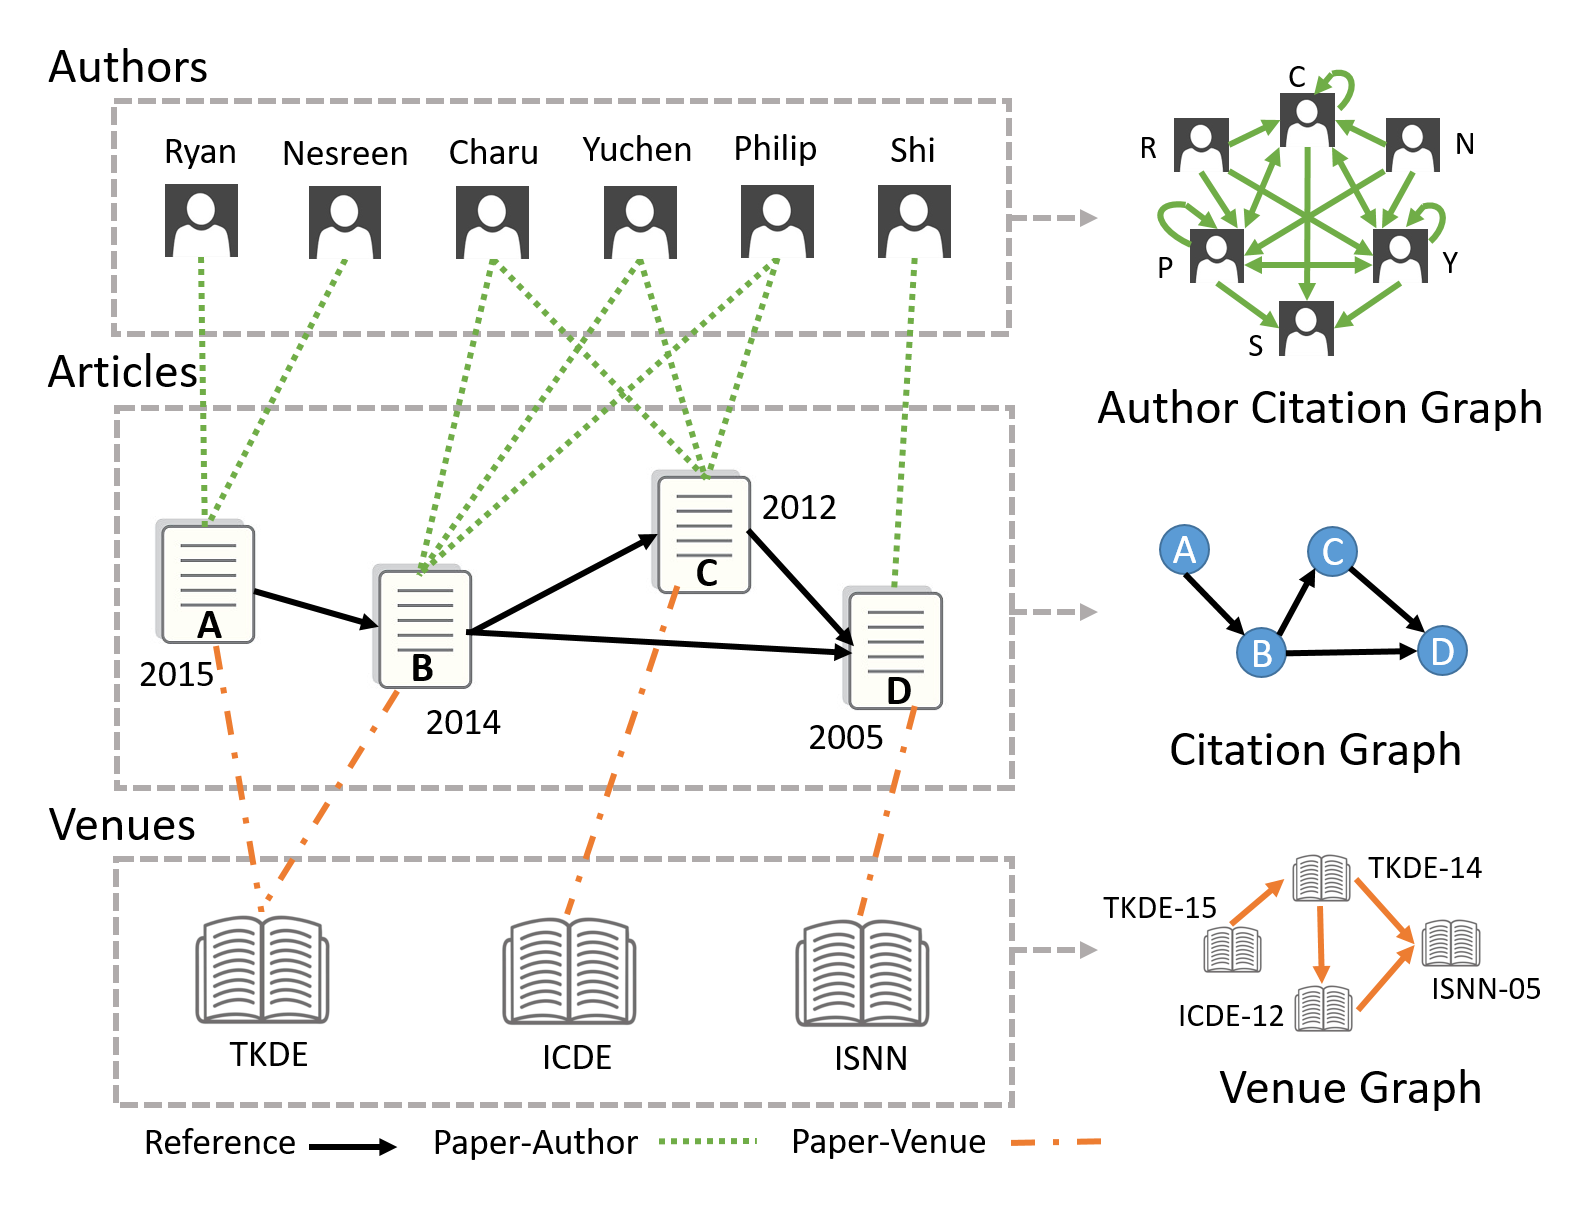
\includegraphics[scale=0.34]{fig/example-graph.eps}
\vspace{-3.3ex}
\caption{\small An example of citation, venue and author citation graphs} \label{fig-example-graph}
\vspace{-3ex}
\end{figure}


\stitle{Venue component}.
The second component computes the importance of venues with their associated articles. As the importance of a venue  evolves with time, we treat the venue in each year individually, and its importance is the sum of importance in all individual years.


A {\em venue graph} $G^v(V^v, E^v)$ is firstly constructed using the citation information among venues such that (a) a node in $V^v$ represents a venue in a specific year, (b) a direct edge $(s,t)$ in $E^v$ denotes that there exist articles published in venue (in a specific year) $s$ citing articles published in venue (in a specific year) $t$, and (c) we use the {\em impact weight} $w_v(s,t)$ to denote the weight  from venues $s$ to $t$, which is the sum of the impact weights from articles published in $s$ to $t$, \ie

\vspace{-1ex}
\begin{small}
\begin{equation} \label{eq-infl-weights-v-app}
w_v(s,t)  = \sum_{u\in C(s), v\in C(t)} w(u,v).
\end{equation}
\end{small}
\noindent
Here, $C(s)$ and $C(t)$ are the sets of articles published in $s$ and $t$, respectively, and $w(u,v)$ is the impact weight of edge $(u, v)$ produced in the citation component.

\begin{example} \label{eg-model-venue}
Recall the heterogeneous academic graph in Fig.~\ref{fig-example-graph}. Its corresponding venue graph is also presented. Note that two nodes in the venue graph are related to venue {\em TKDE} since each node denotes a venue in a specific year. There is an edge from nodes {\em TKDE-15} to {\em TKDE-14} since article A published in {\em TKDE-15} cites article B published in {\em TKDE-14}. And it is similar to derive other edges in the venue graph.
\end{example}

The prestige of a venue in a specific year is computed using the impact weights and the update rule in Eq.~(\ref{eq-twpr}), and the popularity of a venue in a specific year is defined as the average popularity of its articles. The prestige and popularity are combined to derive the importance of a venue in a specific year in the same way as the citation component. Finally, the importance of a venue is treated as the {\em venue importance score} for all articles published in this venue.






\stitle{Author component}.
The author component computes the importance of authors with their published articles.
%
Similar to the venue component, we evaluate the importance of each author, and compute the average importance of the authors of an article as its {\em author importance score}.

%However, the resulting author citation graph to compute the prestige is typically too large to handle.
One way to do this is to construct an author citation graph  such that (a) a node represents an author, and (b) a direct edge $(s,t)$ denotes that there exist articles of author $s$ citing articles of author $t$. However, it is easy to see that for each citation, the corresponding two sets of authors are fully connected, which makes it computationally expensive to compute the prestige of authors on such an author citation graph with TWPageRank.

\begin{example} \label{eg-model-author}
We also include the corresponding author citation graph in Fig.~\ref{fig-example-graph}. Observe that six links in the author citation graph are generated between authors \{{\em Ryan}, {\em Nesreen}\} to \{{\em Charu}, {\em Yuchen}, {\em Philip}\} given a single citation from articles A to B. And it is quite obvious that the number of edges in the author citation graph is much larger than the one in the citation graph, which verifies our claim above.
\end{example}

Hence, we choose to evaluate the prestige of an author with the average prestige of all articles published by the author. Similar to the venue component, the popularity of an author is  defined as the average popularity of her/his published articles. Finally, the prestige and popularity are combined to derive the importance along the same way as the citation component.


\stitle{Ranking with importance assembling}. The aforementioned importance is finally assembled to produce the final ranking, as illustrated in Fig.~\ref{fig-rankmodel}. Before assembling, each component is properly scaled such that the average importance scores of citations, venues and authors are the same.  Let the scaled importance scores of article $v$ be $R_c(v)$, $R_v(v)$, and $R_a(v)$ from the citation, venue and author components, respectively.
%
The final ranking score $R(v)$ is aggregated as follows:

\vspace{-1ex}
\begin{small}
\begin{equation} \label{eq-ensemble-app}
R(v) =  \alpha R_c(v) + \beta R_v(v) + (1 - \alpha - \beta) R_a(v).
\end{equation}
\end{small}
\noindent Here aggregating parameters $\alpha$ and $\beta$ and value $(1 - \alpha - \beta)$ regularize the contributions of the citation, venue and author information,
which make our model be able to fit to the various ranking scenarios. As will be seen in the experiments, our model performs well in two reasonable ranking scenarios by using quite different aggregating parameters, and, moreover, these parameters are indeed quite flexible to choose within a certain range.
Intuitively, these parameters indicate the intensity of the correlation between the importance of scholarly articles and the specific information.



\begin{figure}[tb!]
\centering
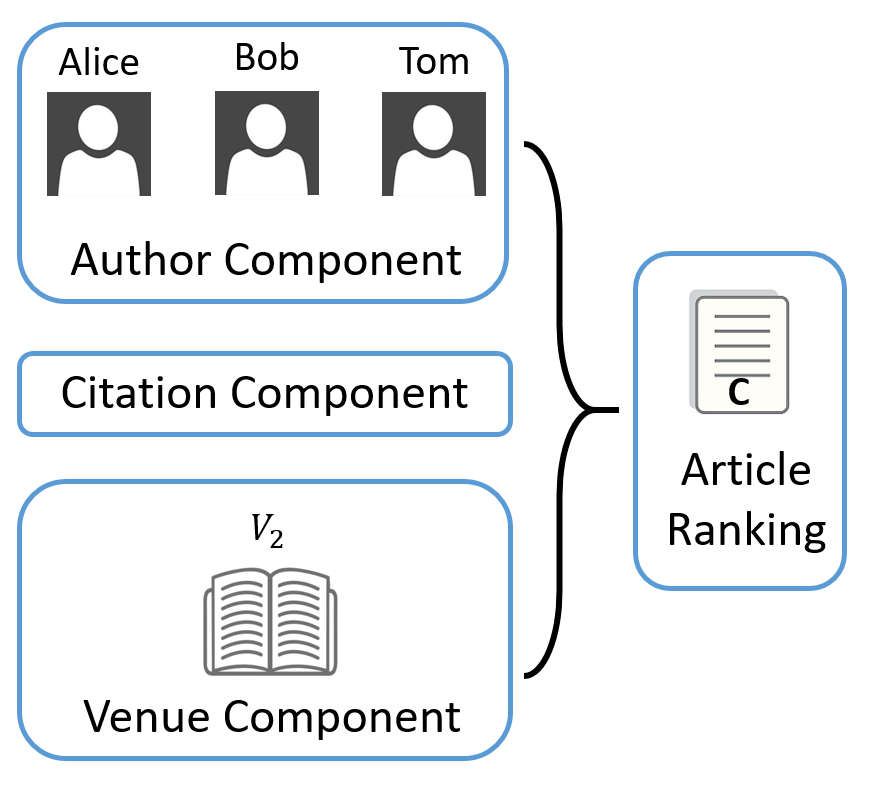
\includegraphics[scale=0.37]{fig/example-ranking.eps}
\vspace{-2ex}
\caption{\small An example of importance assembling} \label{fig-example-ranking}
\vspace{-3ex}
\end{figure}

\begin{example} \label{eg-ranking}
Figure~\ref{fig-example-ranking} illustrates an example of the importance assembling procedure.
Consider an article $v$ published by authors $t$ and $u$ in venue $k$.
(a) It first extracts the importance $c_v$ of article $v$ computed by the  citation component and properly scales $c_v$ to citation importance score $R_c(v)$.
Similarly, (b) it derives the venue importance score $R_v(v)$ based on the venue importance $v_k$ of venue $k$ computed  by the venue component.
(c) The author importance score $R_a(v)$ averages and scales the author importance $a_t$ and $a_u$ of authors $t$ and $u$ computed  by the author component.
Finally, (d) the three importance scores are aggregated to the final ranking score $R(v)$. 
\end{example}


\stitle{Remarks}. This work follows the graph-based formalization, and further develops efficient batch and incremental algorithms based on graphs for scholarly article ranking (Sections~\ref{sec-alg} \& \ref{sec-incAlg}). However, it is also possible to learn a discriminative model that directly optimizes certain loss functions for ranking, similar to \cite{Richardson06:BPR} for ranking Web pages.
